\chapter{Gate-defined triangular cavities}

In this chapter, we simulate a gate defined triangular cavity and describe its operation as a switch that couples different MBS pairs.
The device is built using a stack with three layers of materials: 2DEG, dielectric and metallic gates.
The electrostatic potential inside the 2DEG is found as the solution to Eq. \eqref{eq: laplace} using the finite element solver from Ref. \cite{Armagnat2019}.

Two devices are simulated in order to study the angular dependence previously found.
First, we discuss the tuning of each device such the potential resembles the triangular cavity and the nanowires are strongly coupled.
Then, the MBS coupling is calculated and compared to the purely geometric case.

\section{Gates configuration}

\begin{figure}[h!]
\centering
  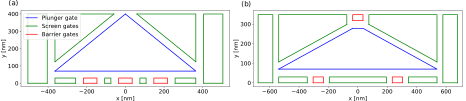
\includegraphics[width=\linewidth]{figures/gate_configurations.pdf}
  \caption{Gate configuration of the two triangular cavities considered. (a) Triangular cavity with angle $\theta = 0.234 \pi$ with all nanowires at the lower side. (b) Triangular cavity with angle $\theta = 0.125\pi$ with central nanowire at the top side. Spacing between gates is set to $40$ nm. Barrier gates have length $30$ nm and width $70$ nm. Nanowires (not shown) are attached at the ends of the barrier gates. The vertical configuration includes a 2DEG of thickness $40$ nm. Then follows an insulating layer of thickness $40$ nm, and finally the metallic gates of thickness $60$ nm.}
  \label{fig:gates}
\end{figure}

A trijunction is a complex Majorana device that can be implemented on a 2DEG by selectively depositing electrostatic gates.
It contains two main regions: three nanowires and a semiconducting cavity.
We focus on the design of a gate defined triangular cavity.
We do not consider the electrostatic modeling of the nanowires since one can assume that the electric field in the nanowires is screened by the superconductor.

The gates are placed in a single layer above the 2DEG with a dielectric layer in between.
Different layer configurations were explored, and a single layer is found to be the best in terms of shape-resolution and voltage range.
The thickness of each layer determines how much the electric field penetrates into the 2DEG.
We consider typical parameters from experiments as described in the inset of Fig. \ref{fig:gates}.

In contrast to the geometrical model discussed in the previous chapter, the trijunction is defined in a smooth potential landscape.
The global potential is affected by all involved gates.
There are three kinds of gates:
\begin{enumerate}
\item Plunger gate: Defines and controls the potential inside the triangular cavity region.
\item Screen gates: There are two kinds of screen gates. First, the triangular screen gates deplete the 2DEG around the plunger gate, which contributes to the overall triangular shape. Second, the screen barrier gates between the tunnel gates that keep each nanowire channel separated from the others.
\item Barrier gates: Modulate the coupling between each nanowire and the cavity. They allow to tune the system in the insulating, tunnelling, and strong coupling regimes.
\end{enumerate}

We envision an operation procedure that is a simple as possible, and therefore we consider an operation that varies the minimum number of gates.
We tune this device by tuning first the barrier gates such that one of the wires remain disconnected.
Then the screen gates in order to deplete the region around the plunger gate.
Finally, we tune the plunger gate in order to probe how different cavity state mediate the MBS coupling.

\section{Device 1}

\begin{figure}
\centering
  \includegraphics[width=\linewidth]{figures/device_1_potential.pdf}
  \caption{Equipotential lines inside the device for representative parameters of the (a) left and right MBS pair and (b) left and center MBS pair. Colorbar indicates value of equipotential lines. (c-d) Cut of the potential along the tunnel barriers, i.e. dashed black lines in (a) and (b), taken for a range of plunger gate voltages. Colorbar in (c-d) indicates the plunger gate voltage.}
  \label{fig:device_1_potential}
\end{figure}

In this section we describe the operation of the gate configuration shown in Fig. \ref{fig:gates} (a).
In Fig.  \ref{fig:device_1_potential} (a) - (b) one can observe the potential inside the 2DEG for the coupling of each pair.
One can observe that the triangular walls are well defined in the potential, but inside the triangle the bottom of the potential has a different shape.

In Fig. \ref{fig:device_1_potential} (c) and (d) one can observe that a double well is created when coupling a given pair of MBS.
For the left and right MBS pair (Fig. \ref{fig:device_1_potential} (c)) the potentials remain well separated.
On the other hand, the central pairs are very close (Fig. \ref{fig:device_1_potential} (d)) and the screen barrier can be lowered below the MBS potential, allowing for direct coupling.

\subsection{Barrier gates tuning}

\begin{figure}
\centering
  \includegraphics[width=\linewidth]{figures/device_1_barriers.pdf}
  \caption{Coupling of (a) left and right MBS pair and (b) left and central MBS pair as a function of the corresponding barrier gates in device 1. Orange lines indicate when the potential at the bottom of the barriers crosses $0$ V. Plunger gate is tuned around the first resonance. Gate voltages used correspond to those described in Table \ref{table:gate_voltages_1}.}
  \label{fig:device_1_barriers}
\end{figure}

Operating the left and right tunnel barriers is straightforward since they are far from each other.
Consequently, there is no interdependence between them as can be observed in Fig. \ref{fig:device_1_barriers} (a).
On the other hand, the operation of the central pairs is not symmetric given the mutual influence of successive barrier gates.
In Fig. \ref{fig:device_1_barriers} (b) one can observe that the slope of the potential crossings suggests a mutual interaction between successive barrier gates.

The system can be tuned in the insulating, tunnelling, and strong coupling regimes by manipulating the barrier gates.
The orange line in Fig. \ref{fig:device_1_barriers} indicate the value of the potential at the bottom of the barrier gates with respect to $0$.
For small voltages, the nanowires are disconnected.
As the voltage increases around the orange line, the system enters into the tunnelling regime.
In this regime, the coupling is mediated by direct overlap of the MBS wavefunctions.
Therefore, one observes a difference in the tunnelling regime of panels (a) and (b) since in the later the MBS are closer.
The orange lines indicate the start of the strong coupling regime.

As the barriers are lowered, there are two new effects:
On one hand, new crossings caused by resonant cavity levels appear.
On the other hand, for very large barrier gates, the MBS couple directly.
The former effect can be seen clearly in panel (a) as the two crossings in the strong coupling regime.
The later can be seen in the lower right part of panel (b) where the coupling increases due to direct coupling.
Keeping the barrier potential as small as possible within strong coupling decreases the influence of these effects.

\subsection{Screen gates tuning}

\begin{figure}
\centering
  \includegraphics[width=\linewidth]{figures/device_1_screens.pdf}
  \caption{Coupling (a) left and right MBS pair and (b) left and central MBS pair as a function of the triangular screen gates in device 1. Three regimes of the depletion are separated by the orange and blue lines. Plunger gate is tuned around the first resonance. Gate voltages used correspond to those described in Table \ref{table:gate_voltages_1}.}
  \label{fig:device_1_screens}
\end{figure}

In Fig. \ref{fig:device_1_screens} one can observe the MBS coupling as a function of the voltages of the two triangular screen gates for each pair.
As mentioned before, these gates deplete the regions surrounding the plunger gate and contribute to the triangular shape resolution.

The triangular screen gates allow to tune the device in three different regimes.
First, in Fig. \ref{fig:device_1_screens} (a) and (b) one observes that below the orange lines, there some resonances with a small MBS coupling.
In this case, electrons can move over the whole 2DEG and are not confined below the plunger gate.
By tuning the potential to more negative values, between the orange and blue lines, a region with large coupling develops, indicating that electrons are confined in the triangular region.
Further increasing the potential depletes the area under the plunger gate as can be seen beyond the blue line, i.e. the plunger gate is depleted.
Observe that higher voltages are required to reach this last regime in Fig. \ref{fig:device_1_screens} (b).

In Fig. \ref{fig:device_1_screens} (a) one observes that the case of the left and right MBS pair is symmetric.
On the other hand, in Fig. \ref{fig:device_1_screens} (b) one observes an asymmetry for the left and central MBS pair.
In fact, the coupling increases by tuning one screen gate more negative than the other.
This is new regime for the coupling of the central MBS pairs that is not found in the purely geometric model.
One can understand this phenomenon as an effectively size decrease for the cavity while maintaining the triangular shape.

\section{Device 2}

\begin{figure}[h!]
\centering
  \includegraphics[width=0.75\linewidth]{figures/device_2_potential.pdf}
  \caption{Equipotential lines inside the device for representative parameters of the (a) left and right MBS pair and (b) left and center MBS pair. Colorbar indicates value of equipotential lines. (c) Cut of the potential along the tunnel barriers, i.e. dashed black lines in (a) and (b), taken for a range of plunger gate voltages. Colorbar in (c) indicates the plunger gate voltage.}
  \label{fig:device_2_potential}
\end{figure}

In this section we describe the operation of the gate configuration shown in Fig. \ref{fig:gates} (b).
In contrast to the previous device, here the interplay between barrier and screen gates is crucial to keep the nanowires connected to the cavity.
In Fig. \ref{fig:device_2_potential} (a) - (b) one can observe the potential inside the 2DEG for connecting each pair.
One observes that the barrier gates are well separated from each other, but the depletion region below the barrier gates depends on the surrounding screen gates as in the case of the top barrier in Fig. \ref{fig:device_2_potential} (b).
Furthermore, in panel (b) one can observe that the potential minima inside the cavity follows a narrow channel trajectory.
The far disconnected end of the triangular potential is higher, which implies a large deformation from the geometrical case.

\subsection{Barrier gates tuning}

\begin{figure}
\centering
  \includegraphics[width=\linewidth]{figures/device_2_barriers.pdf}
  \caption{Coupling (a) left and right MBS pair and (b) left and central MBS pair as a function of the corresponding barrier gates in device 2. Plunger gate is tuned around the first resonance. Gate voltages used correspond to those described in Table \ref{table:gate_voltages_2}.}
  \label{fig:device_2_barriers}
\end{figure}

There are two differences with respect to the previous device:
First, since all barrier gates remain well separated from each other, there is no interdependence of barrier gates for any pair as one can observe in Fig. \ref{fig:device_2_barriers}.
Second, in the tunnelling regime, there is a significant coupling due to wavefunction overlap.
This is a consequence of how the gate geometry influences the spatial distribution of the cavity states.

Since this device has a smaller angle, it resembles a quasi-one dimensional shape.
Observe that the dimension of the plunger gate are $800$ nm long and $200$ nm wide.
The wavefunctions will concentrate around the center of the cavity and not in the narrow edges.
Consequently, one observes a larger coupling in the tunnelling regime due to resonant trapping for the left and right MBS coupling.

In the strong coupling regime (below orange line in Fig. \ref{fig:device_2_barriers}) there is a large difference between the coupling of the different pairs.
One can observe that Fig. \ref{fig:device_2_barriers} (a) is similar to the previous device, which suggests that the triangular geometry effects are present in both devices.
On the other hand, Fig. \ref{fig:device_2_barriers} (b) shows a smaller coupling in contrast to the purely geometric model.
This difference arises from the new structure of the cavity created by the gates.
Furthermore, a new set of resonances appears with a non-trivial dependence in both tunnel barriers.

\subsection{Screen gates tuning}

\begin{figure}[h!]
\centering
  \includegraphics[width=\linewidth]{figures/device_2_screens.pdf}
  \caption{Coupling of (a) left and right MBS pair and (b) left and central MBS pair as a function of the triangular screen gates in device 2. Three regimes of the depletion are separated by the orange and blue lines. Plunger gate is tuned around the first resonance. Gate voltages described in Table \ref{table:gate_voltages_2}.}
  \label{fig:device_2_screens}
\end{figure}

As in the previous device, the coupling is larger when the region around the plunger gate is depleted than when electron delocalise over the 2DEG.
One can observe this in the separate regions shown in Fig. \ref{fig:device_2_screens} marked by the blue and orange lines.
In Fig. \ref{fig:device_2_screens} (a) one observes that there is a region where the coupling for the left and right MBS pair has a series of large resonances.
By tuning the screen gates inside one of them, the magnitude of the coupling is similar to the previous device.

As mentioned before, the position of the barrier gates is modulated by the screen gates.
One can observe in Fig. \ref{fig:device_2_screens} (a) that for voltages above the blue line one of the nanowires disconnects from the cavity.
On the other hand, in in Fig. \ref{fig:device_2_screens} (b) one observes the dependence on the screen gates is asymmetric.
In this case, the right screen gate disconnects the top nanowire at a voltage smaller than the lower gates.
Finally, the region below the orange lines indicates that there is a non-zero coupling for when electrons delocalised over the 2DEG, but no distinguishable pattern is found.

In this device is possible to reach a maximum coupling by properly tuning the screen and barrier gates.
The gates design does not allow to explore cases beyond the triangular cavity as in the previous device.
In fact, tuning of the screen gates is required for each pair to operate properly.

\section{Devices operation}

In the previous discussion we have described the optimal point for operating each the devices considered.
In this section we tune the devices to the operational point described in Tables \ref{table:gate_voltages_1} anad \ref{table:gate_voltages_2}.
Then we calculate the MBS coupling as a function of the plunger gate and the result is shown in Fig. \ref{fig:devices_coupling}.
By observing Fig. \ref{fig:devices_coupling} (a), we can see that the coupling of the different MBS pairs is close to the maximum coupling around $V_{plunger}=2$meV for the first device.
On the other hand, Fig. \ref{fig:devices_coupling} (b) shows that the coupling of different pairs in the second device is highly asymmetric.
A maximum can be found for all pairs around $V_{plunger} = 6.5$ meV.
However, there is a difference of about $30$ meV for the coupling of different pairs in this device.

The shape of the spectra for both MBS pairs in device 1 (Fig. \ref{fig:devices_coupling} (a)) is similar, but the central pair has a larger level spacing.
This support the idea that the deformation of the triangular cavity leads to an effective size reduction that involves only the relevant pairs.
On the other hand, in Fig. \ref{fig:devices_coupling} (b) one observes a region where the coupling has a peak for the left and right pair, but it has a dip for central pairs.

\begin{figure}[h!]
\centering
  \includegraphics[width=0.8\linewidth]{figures/device_couplings.pdf}
  \caption{MBS coupling of all relevant pairs for each device tuned accordingly to the parameters described in Table \ref{table:gate_voltages_1} and Table \ref{table:gate_voltages_2}.}
  \label{fig:devices_coupling}
\end{figure}

Both devices are operated by changing three gate voltages at a time to tune between each MBS pair.
First of all, the barrier gates are required to connect or disconnect nanowires from the cavity.
Tuning between different pairs requires to disconnect one wire while connect a new one.
The largest voltage difference in the tuning comes from the barrier gates.
Then, the screen gates are tuned such that the region around the plunger gate is depleted.
Further tuning for the central pairs is required as was discussed in Fig. \ref{fig:device_1_screens} (b).
The set of gate voltages that define the operational point of the devices are shown in Table \ref{table:gate_voltages_1} and Table \ref{table:gate_voltages_2}.

\begin{table}[h!]
\centering
\begin{tabular}{||c ||c c c c c ||} 
 \hline
& $V_{barrier}^L$ & $V_{barrier}^R$ & $V_{barrier}^C$ & $V_{screen}^L$ & $V_{screen}^R$ \\
 \hline\hline
 left-right & 35 & 35 & -20 & -15 & -15\\ 
 \hline
 left-center & 35 & -20 & 20 & -15 & 40\\ 
 \hline
 center-right & -20 & 35 & 20 & 40 & -15\\ 
 \hline
 \hline
\end{tabular}
\caption{Optimal gate configuration of device 1 shown in Fig. \ref{fig:gates}(a). Voltage units are $meV$. Remaining gate voltages are fixed: screen barriers between nanowires $-30$ meV, screen barriers around nanowires $-15$ meV.}
\label{table:gate_voltages_1}
\end{table}

\begin{table}[h!]
\centering
\begin{tabular}{||c ||c c c c c ||} 
 \hline
&  $V_{barrier}^L$ & $V_{barrier}^R$ & $V_{barrier}^C$ & $V_{screen}^L$ & $V_{screen}^R$ \\
 \hline\hline
 left-right & 17 & 17 & -20 & -15 & -15\\ 
 \hline
 left-center  & 17 & -20 & 17 & -10 & -20\\ 
 \hline
 center-right & -20 & 17 & 17 & -20 & -10\\ 
 \hline
 \hline
\end{tabular}
\caption{Optimal gate configuration of device 2 shown in Fig. \ref{fig:gates}(b). Voltage units are $meV$. Remaining gate voltages are fixed: screen barriers between nanowires $-30$ meV, screen barriers around nanowires $-15$ meV.}
\label{table:gate_voltages_2}
\end{table}



